\section{Prerequisiti}
\subsection{Alfabeto greco}
    \begin{table}[h]
    \centering
    \label{tab:alfabeto_greco}
    \begin{minipage}{0.32\textwidth} % Colonna 1
        \centering
        \begin{tabular}{ll}
            Alfa & $\alpha$ A \\
            Beta & $\beta$ B \\
            Gamma & $\gamma$ $\Gamma$ \\
            Delta & $\delta$ $\Delta$ \\
            Epsilon & $\epsilon$ E \\
            Zeta & $\zeta$ Z \\
            Eta & $\eta$ H \\
            Theta & $\theta$ $\Theta$ \\
        \end{tabular}
    \end{minipage}
    \hfill
    \begin{minipage}{0.32\textwidth} % Colonna 2
        \centering
        \begin{tabular}{ll}
            Iota & $\iota$ I \\
            Kappa & $\kappa$ K \\
            Lambda & $\lambda$ $\Lambda$ \\
            Mu (Mi) & $\mu$ M \\
            Nu (Ni) & $\nu$ N \\
            Xi & $\xi$ $\Xi$ \\
            Omicron & o O \\
            Pi & $\pi$ $\Pi$ \\
        \end{tabular}
    \end{minipage}
    \hfill
    \begin{minipage}{0.32\textwidth} % Colonna 3
        \centering
        \begin{tabular}{ll}
            Rho & $\rho$ P \\
            Sigma & $\sigma$ $\Sigma$ \\
            Tau & $\tau$ T \\
            Upsilon & $\upsilon$ Y \\
            Phi & $\phi$ $\Phi$ \\
            Chi & $\chi$ X \\
            Psi & $\psi$ $\Psi$ \\
            Omega & $\omega$ $\Omega$ \\
        \end{tabular}
    \end{minipage}
    \caption{Tabella dell'alfabeto greco}
\end{table}

\subsection{Logica}
    \subsubsection{Proposizioni}
        Una proposizione è un'affermazione alla quale si può assegnare un valore di verità o falsità, ma non entrambi contemporaneamente. In altre parole, una proposizione è un enunciato con un valore di verità ben definito. Le proposizioni costituiscono la base della logica matematica e sono utilizzate per formulare teoremi, lemmi e corollari.
    
        In logica formale, una proposizione può essere rappresentata mediante una variabile proposizionale, come \( p \), \( q \), o \( r \). Ogni variabile proposizionale rappresenta un enunciato che può essere classificato come vero o falso. Queste variabili possono essere combinate utilizzando diversi operatori logici per formare proposizioni più complesse e costruire argomentazioni logiche:
    
        \begin{enumerate}
            \item \textbf{Negazione}:
                \begin{flushleft}
                    \(\neg\), si legge \underline{non} \\
                    \(\neg p\), si legge \underline{non \( p \)}
                \end{flushleft}
                \vspace{1em} 
                \underline{Esempio:} \( p \): Trieste è una città francese. (\(\neg p\)) \\
    
                Il comportamento di un connettivo logico è stabilito dalla tabella di verità. \\
    
                \begin{table}[h!]
                    \centering
                    \begin{tabular}{|c|c|}
                        \hline
                        $p$ & $\neg p$ \\
                        \hline
                        V & F \\
                        F & V \\
                        \hline
                    \end{tabular}
                    \caption{Tabella di verità per $p$ e $\neg p$.}
                \end{table}
        
            \item \textbf{congiunzione}: 
                \begin{flushleft}
                    \(\land\) si legge \underline{e} \\
                   \( p \)\(\land\)\( q \), si legge \underline{\( p \) e \( q \)}
                \end{flushleft}
    
                \begin{table}[h!]
                    \centering
                    \begin{tabular}{|c|c|c|}
                        \hline
                        $p$ & $q$ & $p \land q$ \\
                        \hline
                        V & V & V \\
                        V & F & F \\
                        F & V & F \\
                        F & F & F \\
                        \hline
                    \end{tabular}
                    \caption{Tabella di verità per $p \land q$.}
                \end{table}
    
            \item \textbf{disgiunzione}: 
               \begin{flushleft}
                    \(\lor\), si legge \underline{o} \\
                    \( p \lor q \), si legge \underline{\( p \) o \( q \)}
                \end{flushleft}
                
                \begin{table}[h!]
                    \centering
                    \begin{tabular}{|c|c|c|}
                        \hline
                        $p$ & $q$ & $p \lor q$ \\
                        \hline
                        V & V & V \\
                        V & F & V \\
                        F & V & V \\
                        F & F & F \\
                        \hline
                    \end{tabular}
                    \caption{Tabella di verità per \( p \lor q \).}
                \end{table}
                
                \newpage
                
                La disgiunzione non è esclusiva; è possibile trovare un rapporto tra questi connettivi. In particolare, possiamo trovare due modi equivalenti per esprimere:
                
                \begin{center}
                    \(\neg (p \land q)\) \\
                    \(\neg (p \lor q)\)
                \end{center}
                
                Le leggi di De Morgan stabiliscono le seguenti equivalenze:
                
                \[\neg (p \land q) \equiv (\neg p \lor \neg q)\]
                
                \begin{table}[h!]
                    \centering
                    \begin{tabular}{|c|c|c|c|c|c|c|}
                        \hline
                        $p$ & $q$ & $p \land q$ & $\neg (p \land q)$ & $\neg p$ & $\neg q$ & $\neg p \lor \neg q$ \\
                        \hline
                        V & V & V & F & F & F & F \\
                        V & F & F & V & F & V & V \\
                        F & V & F & V & V & F & V \\
                        F & F & F & V & V & V & V \\
                        \hline
                    \end{tabular}
                    \caption{Tabella di verità per \(\neg (p \land q) \equiv (\neg p \lor \neg q)\).}
                \end{table}
                
                \vspace{1em} 
                
                \[\neg (p \lor q) \equiv (\neg p \land \neg q)\]
                
                \begin{table}[h!]
                    \centering
                    \begin{tabular}{|c|c|c|c|c|c|c|}
                        \hline
                        $p$ & $q$ & $p \lor q$ & $\neg (p \lor q)$ & $\neg p$ & $\neg q$ & $\neg p \land \neg q$ \\
                        \hline
                        V & V & V & F & F & F & F \\
                        V & F & V & F & F & V & F \\
                        F & V & V & F & V & F & F \\
                        F & F & F & V & V & V & V \\
                        \hline
                    \end{tabular}
                    \caption{Tabella di verità per \(\neg (p \lor q) \equiv (\neg p \land \neg q)\).}
                \end{table}
    
    
            \item \textbf{implicazione}: 
                \begin{flushleft}
                     L'implicazione \( p \implies q \) è vera in tutti i casi tranne quando \( p \) è vero e \( q \) è falso.
                    \( p \implies\ q \), si legge \underline{se \( p \) allora \( q \)}, \underline{\( p \) implica \( q \)}
                \end{flushleft}
    
                \begin{table}[h!]
                    \centering
                    \begin{tabular}{|c|c|c|}
                        \hline
                        $p$ & $q$ & $p \implies q$ \\
                        \hline
                        V & V & V \\
                        V & F & F \\
                        F & V & V \\
                        F & F & V \\
                        \hline
                    \end{tabular}
                    \caption{Tabella di verità per \( p \implies q \).}
                \end{table}
            
        \end{enumerate} \newpage
    
        \vspace{1em} 
        \underline{Doppia Negazione}: \\
        L'implicazione logica \( p \implies q \) è equivalente alla disgiunzione di \( \neg p \) e \( q \), in simboli:
        \[
        p \implies q \equiv \neg p \lor q
        \]
        La negazione dell'implicazione, \( \neg (p \implies q) \), è equivalente a \( p \land \neg q \). In simboli:
        \[
        \neg (p \implies q) \equiv p \land \neg q
        \]
    
        \begin{table}[h!]
            \centering
            \begin{tabular}{|c|c|c|c|c|}
                \hline
                $p$ & $q$ & $\neg p$ & $p \implies q$ & $\neg p \lor q$ \\
                \hline
                V & V & F & V & V \\
                V & F & F & F & F \\
                F & V & V & V & V \\
                F & F & V & V & V \\
                \hline
            \end{tabular}
        \end{table}
                                                           
                                                           
        \textbf{Doppia implicazione}:    \\
         Il bicondizionale, rappresentato con \( p \iff q \), è vero se e solo se entrambe le proposizioni sono entrambe vere o entrambe false. Si legge \underline{\( p \) se e solo se \( q \)}.
        
    
    
        \begin{table}[h!]
            \centering
            \begin{tabular}{|c|c|c|}
                \hline
                $p$ & $q$ & $p \iff q$ \\
                \hline
                V & V & V \\
                V & F & F \\
                F & V & F \\
                F & F & V \\
                \hline
            \end{tabular}
            \caption{Tabella di verità per $p \iff q$.}
        \end{table}
    
        Di conseguenza il bicondizionale può essere espresso come la combinazione di due implicazioni: \\
        \[p \iff q = (p \implies q)\land(q \implies p)\]    \\
        
        \begin{table}[h!]
            \centering
            \begin{tabular}{|c|c|c|c|c|}
            \hline
            $p$ & $q$ & $p \implies q$ & $q \implies p$ & $(p \implies q) \land (q \implies p)$ \\
                \hline
                V & V & V & V & V \\
                V & F & F & V & F \\
                F & V & V & F & F \\
                F & F & V & V & V \\
                \hline
            \end{tabular}
            \caption{Tabella di verità per $p \iff q = (p \implies q) \land (q \implies p)$.}
        \end{table}
    
        
        \underline{Esempio:} \\
        $p$: in un triangolo, 2 lati sono uguali.     \\
        $q$: in un triangolo, 2 angoli sono uguali.   \\
        \(p \iff q\)

    \newpage

    \subsubsection{Predicati}
        Sono parte del nostro ragionamento in cui compaiono 1 o più variabili

        \vspace{1em} 
        
        $P(x)$ Lo studente $x$ è alto più di 1,80m.    \\
        A seconda del valore di $x$ il predicato è vero o falso. Per un valore assegnato a $x$ il predicato diventa una proposizione.   \\

        Un predicato può essere: \\
        \begin{itemize}
            \item \underline{unario} una variabile $P(x)$
            \item \underline{binario} due variabili $Q(x,y)$
        \end{itemize}

    \subsubsection{Quantificatori}
    I quantificatori ci permettono di fare affermazioni riguardo a tutti o alcuni elementi di un insieme. Esistono due quantificatori principali nella logica:

    \begin{enumerate}
        \item \textbf{Quantificatore universale}    \\
        \vspace{1em} 
        $\forall x,P(x)$ si legge \underline{Per ogni $x$, vale $p(X)$} \\
        \underline{Esempio:}    \\
        $P(x)$: Lo studente è più alto di 1,8m. \\
        \(\forall x,P(x)\) ogni studente è più alto di 1,8m.
            
        \item \textbf{Quantificatore esistenziale}  \\
        \vspace{1em} 
        $\exists x:P(x)$ si legge \underline{esiste (almeno) un $x$ per cui vale $P(x)$.}   \\ 
        \underline{Esempio:}    \\
        $P(x)$: Lo studente è più alto di 1,8m. \\
        $\exists x:P(x)$ Almeno uno studente è più alto di 1,8m.
    \end{enumerate}

    \textbf{Relazione tra quantificatori:}  \\
    \vspace{0,5em}
    $Q(x,y)$= Astronomo x osserva la stella y.  \\
    $\forall x,Q(x,y)$= Tutti gli astronomi osservano la stella y.  \\
    $\forall x,\exists y,Q(x,y)$= Per ogni astronomo c'è una stella che viene osservata.    \\
    $\exists x: \forall y,Q(x,y)$= C'è un astronomo che osserva tutte le stelle.    \\

    \vspace{1em}
    \textbf{Come si nega frase con un quantificativo?}  \\
    Ogni studente è più alto di 1,8m.   \\
    \underline{Come si nega?}   \\
    C'è almeno uno studente più basso di 1,8m.  \\
    \begin{center}
        \(\neg(\forall x,P(x))=\exists x:\neg P(x)\)    \\
        \(\neg(\exists x:Q(x))=\forall x:\neg Q(x)\)    
    \end{center}

    \underline{esempio:}    \\
    $Q(x,y)$ astronomo $x$ osserva stella $y$.  \\
    \(\forall x, \exists y:Q(x,y)\) Per ogni astronomo $x$, esiste almeno una stella $y$ tale che $x$ osserva $y$.
        
    \begin{center}
        \begin{tabular}{r l}
            \(\forall x,(\exists y: Q(x,y))\) & \textit{Ogni astronomo osserva almeno una stella.} \\
            \(\neg (\forall x,\exists y: Q(x,y))\) & \textit{Esiste almeno un astronomo che non osserva nessuna stella.} \\
            \(\exists x:\neg(\exists y:Q(x,y))\) & \textit{Esiste un astronomo che non osserva alcuna stella.} \\
            \(\exists x: \forall y, \neg Q(x,y)\) & \textit{Esiste un astronomo che non osserva nessuna stella.}
        \end{tabular}
    \end{center}

\newpage
\subsection{Insiemi}
Un insieme è una nozione primitiva che si riferisce a una collezione (o famiglia) di oggetti, detti \underline{elementi dell'insieme}. Gli insiemi sono uno dei concetti fondamentali della matematica e vengono utilizzati per descrivere collezioni di oggetti ben definiti, che possono essere di qualsiasi tipo, come numeri, persone, lettere o altri insiemi.

Indichiamo un insieme con una lettera maiuscola, ad esempio \( A \), \( B \), \( C \), mentre gli elementi dell'insieme sono indicati con lettere minuscole, come \( a \), \( b \), \( c \), ecc.

\subsubsection{Appartenenza}
L'appartenenza di un elemento a un insieme viene indicata con il simbolo \( \in \). Se un elemento \( a \) appartiene all'insieme \( A \), si scrive:
\[
a \in A
\]
Se invece l'elemento \( a \) non appartiene all'insieme \( A \), si scrive:
\[
a \notin A
\]

\subsubsection{Insiemi Finiti e Infiniti}
Gli insiemi possono essere finiti o infiniti. Un insieme è detto finito se contiene un numero finito di elementi; altrimenti, è detto infinito. Ad esempio:
\[
A = \{1, 2, 3, 4\}
\]
è un insieme finito, mentre:
\[
B = \{1, 2, 3, \dots\}
\]
è un insieme infinito, poiché contiene tutti i numeri naturali.

\subsubsection{Sottoinsiemi}
Se $A$ e $B$ sono insiemi e tutti gli elementi di $A$ sono anche elementi di $B$, dirò che: \[A \subseteq B\]

\textbf{attenzione!}    \\
$\in$ appartiene (si parla di elementi)   \\
è diverso da    \\
$\subseteq$ è contenuto di (si parla di insiemi)  \\
\begin{figure}[h!]
    \centering
    \begin{minipage}{0.8\textwidth}
        \centering
        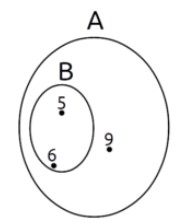
\includegraphics[width=0.2\textwidth]{img/chap_1/contenuto_appartenenza.jpg}
    \end{minipage}%
    \begin{minipage}{0.5\textwidth}
        \raggedright % Testo allineato a sinistra
        \( B \subseteq B \) \\[1em]
        \( 5 \in B \)
    \end{minipage}
    \caption{Relazione tra insiemi e appartenenza.}
\end{figure}

\vspace{1em}
Se $A\subseteq B$ diro che $A$ è sottoinsieme di $B$.   \\
\vspace{1em}
vale $A=B\iff A\subseteq B\land B\subseteq A$   \\
Esiste un'insieme che non ha elementi, lo chiamiamo insieme vuoto e lo segnamo come $\emptyset$.    \\
Ho $\forall A$ insieme, $\emptyset \subseteq A$ \\
Il vuoto è unico!

\subsubsection{Operazioni tra Insiemi}
\begin{enumerate}
    \item \textbf{Unione}: L'unione di due insiemi \( A \) e \( B \), denotata con \( A \cup B \), è l'insieme di tutti gli elementi che appartengono ad \( A \), \( B \) o a entrambi.
    \[A \cup B = \{x \, | \, x \in A \, \text{oppure} \, x \in B\}
    \]
    
    \item \textbf{Intersezione}: L'intersezione di due insiemi \( A \) e \( B \), denotata con \( A \cap B \), è l'insieme di tutti gli elementi che appartengono sia ad \( A \) sia a \( B \).
    \[
    A \cap B = \{x \, | \, x \in A \, \text{e} \, x \in B\}
    \]
    
    \item \textbf{Differenza}: La differenza tra due insiemi \( A \) e \( B \), denotata con \( A \setminus B \), è l'insieme di tutti gli elementi che appartengono ad \( A \) ma non a \( B \).
    \[
    A \setminus B = \{x \, | \, x \in A \, \text{e} \, x \notin B\}
    \]
    \end{enumerate}
\begin{center}
     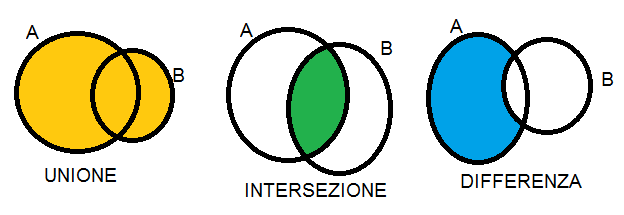
\includegraphics[width=0.6\textwidth]{img/chap_1/unione_intersezione_differenza.png}
\end{center}



    

    
    
    
